\documentclass[12pt]{article}

% Language setting
% Replace `english' with e.g. `spanish' to change the document language
\usepackage[czech]{babel}

% Set page size and margins
% Replace `letterpaper' with `a4paper' for UK/EU standard size
\usepackage[a4paper ,top=2cm,bottom=2cm,left=2.5cm,right=2.5cm,marginparwidth=1.75cm]{geometry}

% Useful packages
\usepackage{amsmath}
\usepackage{graphicx}
\usepackage{float}
\usepackage{setspace}
\usepackage{amsmath}
\usepackage[colorlinks=true, allcolors=blue]{hyperref}

\begin{document}
\onehalfspacing
\begin{center}
    {
\includegraphics[width=0.7\linewidth]{logo_cz.png}}\\[50pt]
    {\Huge Vysoké Učení Technické v Brně}\\[10pt]
    {\huge Fakulta Informačních Technologií}\\[150pt]
    {\Huge \textbf{Mikroprocesorové a vestavěné systémy}}\\[15pt]
    {\huge Měření teploty}\\[225pt]
    \noindent
    \makebox[\textwidth]{
        \Large Nikita Smirnov, xsmirn02
        \hfill
        \Large 15. prosince 2024
    }
\end{center}
\newpage

% \tableofcontents
% \newpage

\section {Úvod}
Cílem tohoto projektu je implementovat program pro měření teploty pomocí analogového čidla. \\
Program zpracovává každou sekundu přijatý signál z teplotního čidla a převádí jej na skutečnou teplotu. Naměřená teplota je poté odeslána do brokeru mqtt a uložena do nvs.\\
Hlavním cílem bylo vytvořit funkční, snadno rozšiřitelný a udržovatelný kód. Toho bylo dosaženo rozdělením programu do modulů, které jsou řízeny ze souboru main.c.

Videoprezentace funkčnosti projektu: \href{https://youtu.be/4n5uWdhA3MM?si=1hYrYChPR6tf-U4K}{video}

\subsection{Použité nástroje}
\begin{itemize}
    \item \textbf{Programovací jazyk} - C.
    \item \textbf{Prostředí} - ESP-IDF.
    \item \textbf{Deska} - Wemos D1 R32(ESP32).
    \item \textbf{Teplotní čidlo} - LMT85LPG.
    \item \textbf{IDE} - PlatformIO IDE for VSCode.
\end{itemize}

\section {Implementace}
Program je rozdělen do několika modulů, které obsahují realizaci konkrétních částí projektu:
\begin{itemize}
    \item \textbf{$main.c$} - Odpovídá za řízení hlavní smyčky programu. Rovněž inicializuje komponenty.
    \item \textbf{$config.h$} - Obsahuje nastavení pro provoz programu a definuje konfigurační strukturu pro jeho další načítání z paměti nebo konfigurační stránky.
    \item \textbf{$memory\_handler.h$} - Inicializuje a odpovídá za práci s perzistentní pamětí, včetně logiky načítání konfigurace projektu.
    \item \textbf{$mqtt\_handler.h$} - Inicializuje spojení s mqtt brokerem, je zodpovědný za zpracování informací přijatých ze serveru a odesílání dat na server. V současné době podporuje pouze připojení přes TCP.
    \item \textbf{$temp\_sensor.h$} - Odpovídá za řízení provozu teplotního čidla. Obsahuje také funkce pro získávání napětí a jejich převod na stupně. Vzhledem k tomu, že informace jsou přijímány ne častěji než jednou za sekundu, byla zvolena metoda využívající $esp\_adc/adc\_oneshot.h$
    \item \textbf{$threshold.h$} - Funkce byla vyhrazena do samostatného modulu, protože má potenciál pro rozšíření, nicméně v současné době pouze přepínáme diodu v závislosti na konfiguraci prahového tepla a hysterezi.
    \item \textbf{$wifi\_handler.h$} - Odpovídá za inicializaci a zpracování událostí, které jsou generovány během připojení k wifi.
\end{itemize}


\section {Spuštění}
\subsection{Zapojení}
\subsubsection{Deska}
Používáme desku Wemos D1 R32. V našem případě používáme porty GPIOP2(ADC12) pro připojení diody a GPIOP39(ADC3) pro čtení teplotního čidla. Tyto porty lze samozřejmě v konfiguraci($config.h$) změnit. \\
{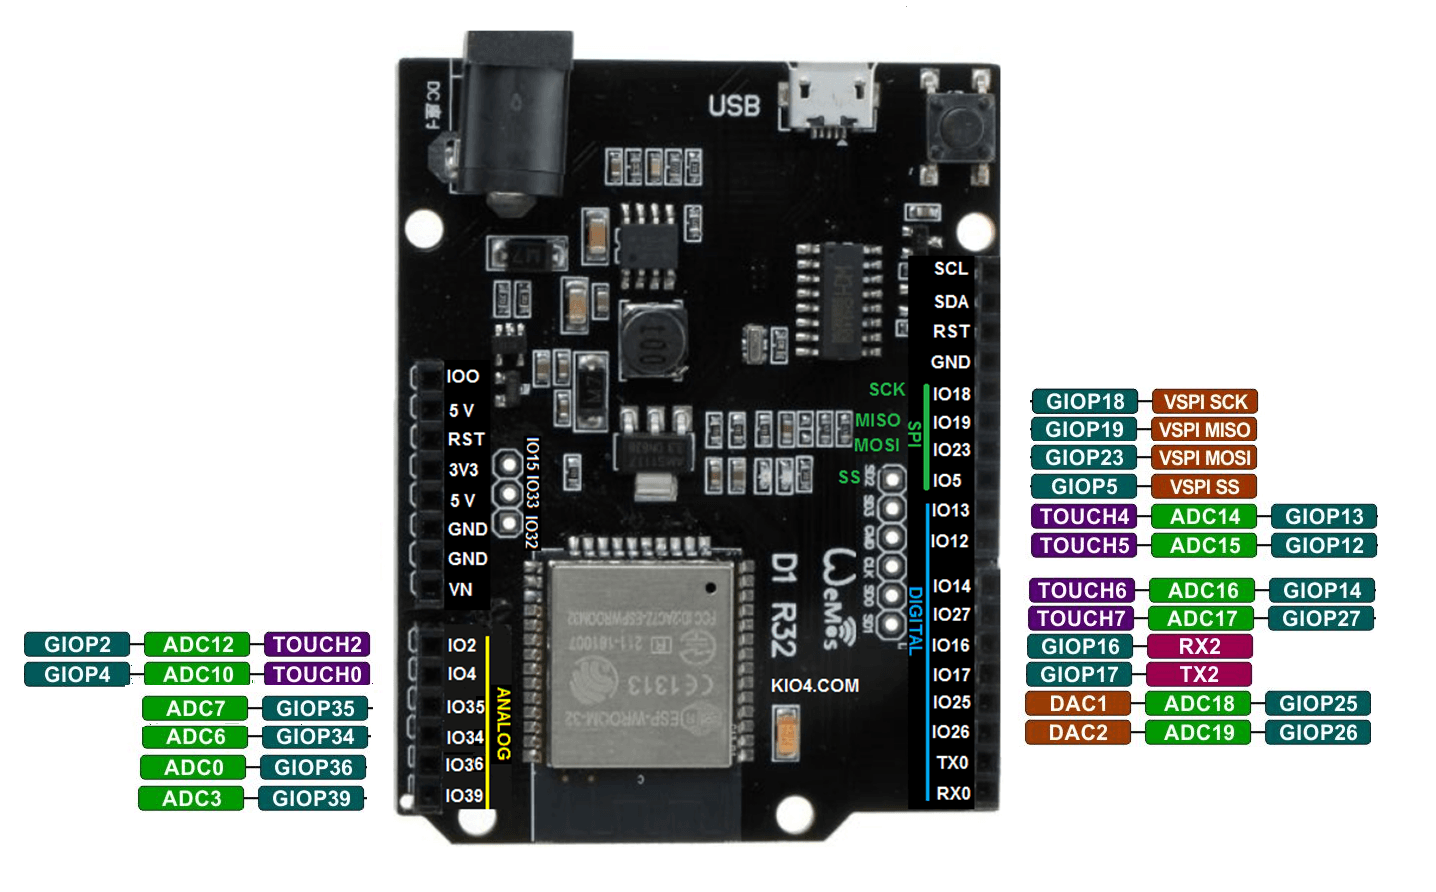
\includegraphics[width=0.7\linewidth]{wemos.png}}\\[50pt]

\subsubsection{Teplotní čidlo}
Používáme teplotní čidlo LMT85LPG(TO-92S) pro 3.3V\\
{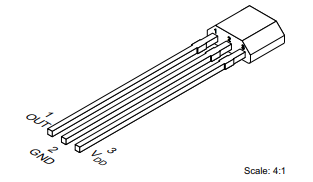
\includegraphics[width=0.4\linewidth]{lmt85.png}}\\[50pt]

\subsubsection{Celkový pohled na připojení}
{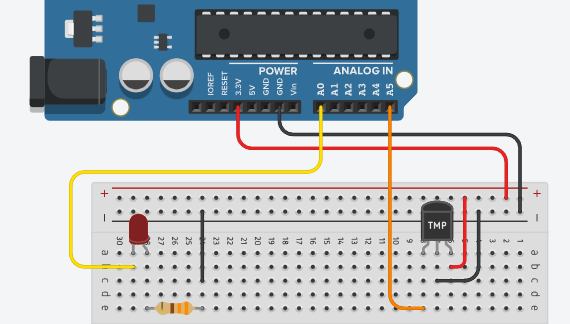
\includegraphics[width=0.7\linewidth]{zap.png}}\\[50pt]


\subsection{Nastavení}
Konfigurace se provádí přes  konfigurační stránku(menuconfig $->$ Temperature controller). Pokud není zadána žádná konfigurace, program se pokusí převzít hodnotu, která byla uložena v nvs. Pokud tato hodnota není přítomna, bude program pracovat s omezeními (např. nebude odesílat informace do mqtt brokeru).\\
{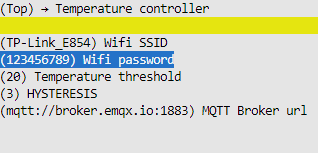
\includegraphics[width=0.7\linewidth]{menuconfig.png}}\\[50pt]

\subsubsection{Nastavení debug}
V souboru main.c můžete nastavit debug = 1 pro zobrazení ladicích informací.

\subsubsection{Nastavení wifi}
Zadejte SSID a heslo sítě, ke které se chcete připojit. Upozorňujeme však, že se nelze připojit k sítím 5G.

\subsubsection{Nastavení temperature threshold a hysteresis}
Můžete zadat teplotní limit pro provedení modulu threshold.h a také hysterezi.
Program také umožňuje aktualizovat tyto hodnoty pomocí MQTT, a to tak, že se program přihlásí k odběru témat:
\begin{itemize}
    \item $xsmirn02/temp\_threshold$ 
    \item $xsmirn02/temp\_hysteresis$ 
\end{itemize}
Tyto hodnoty lze aktualizovat jednoduše zasláním požadavku obsahujícího pouze novou hodnotu do spojeného tématu.

\subsubsection{Nastavení MQTT broker url}
Zadejte brokera pro použití MQTT, pokud není broker zadán, program bude pokračovat bez použití MQTT. Je třeba poznamenat, že program pracuje s brokery MQTT pouze prostřednictvím připojení TCP.


% \bibliographystyle{alpha}
% \bibliography{sample}

\end{document}